%
% Chapter 4
%
\chapter {Shor's Semiprime Integer Factorization Algorithm}

Shor's algorithm is a polynomial-time quantum algorithm for semiprime integer factorization. In comparison, the time complexity of the most efficient known classical factoring algorithm is superpolynomial.

We chose Shor's algorithm because it is one of the most significant quantum algorithms due to its exponential improvement on efficiency compared to its classical counterparts, and because both the number of qubits and the number of quantum operations required to run it are proportional to the input size. The number of operations is particullarly relevant since it makes the errors introduced by the physical gates an important consideration.

\section{Algorithm}

The problem that Shor's algorithm solves is the following: given a semiprime integer \textit{N}, find its two prime factor \textit{p} and \textit{q}.

Shor's algorithm combines both classical and quantum computations, and the procedure to perform it is the following:
\begin{enumerate}
    \item Pick a random integer $1 < a < N$.
    \item Check whether $a$ is a factor by determining whether $a$ and $N$ are comprime. If they are, we can compute the factors. Otherwise continue with the rest of the algorithm.
    \item Use a period-finding quantum subroutine to find the period $r$ of the function $f(x)=a^{x} \ mod \ N$.
    \item If $r$ is odd, then go back to step 1. If $r$ is even, go to the next step.
    \item If $a^{\frac{r}{2}} \equiv -1  \ mod \ N$, then go back to step 1.
    \item Either $a^{\frac{r}{2}} - 1$ or $a^{\frac{r}{2}} + 1$ shares a factor with $N$.
\end{enumerate}

Figure \ref{fig:PeriodFindingQuantumSubroutine} shows the circuit that implements the quantum subroutine in Shor's algorithm. The quantum circuits $Ua^{2^k}$ used for this algorithm are custom designed for each value of $N$ and $a$.

\begin{figure}[h!]
    \centering
    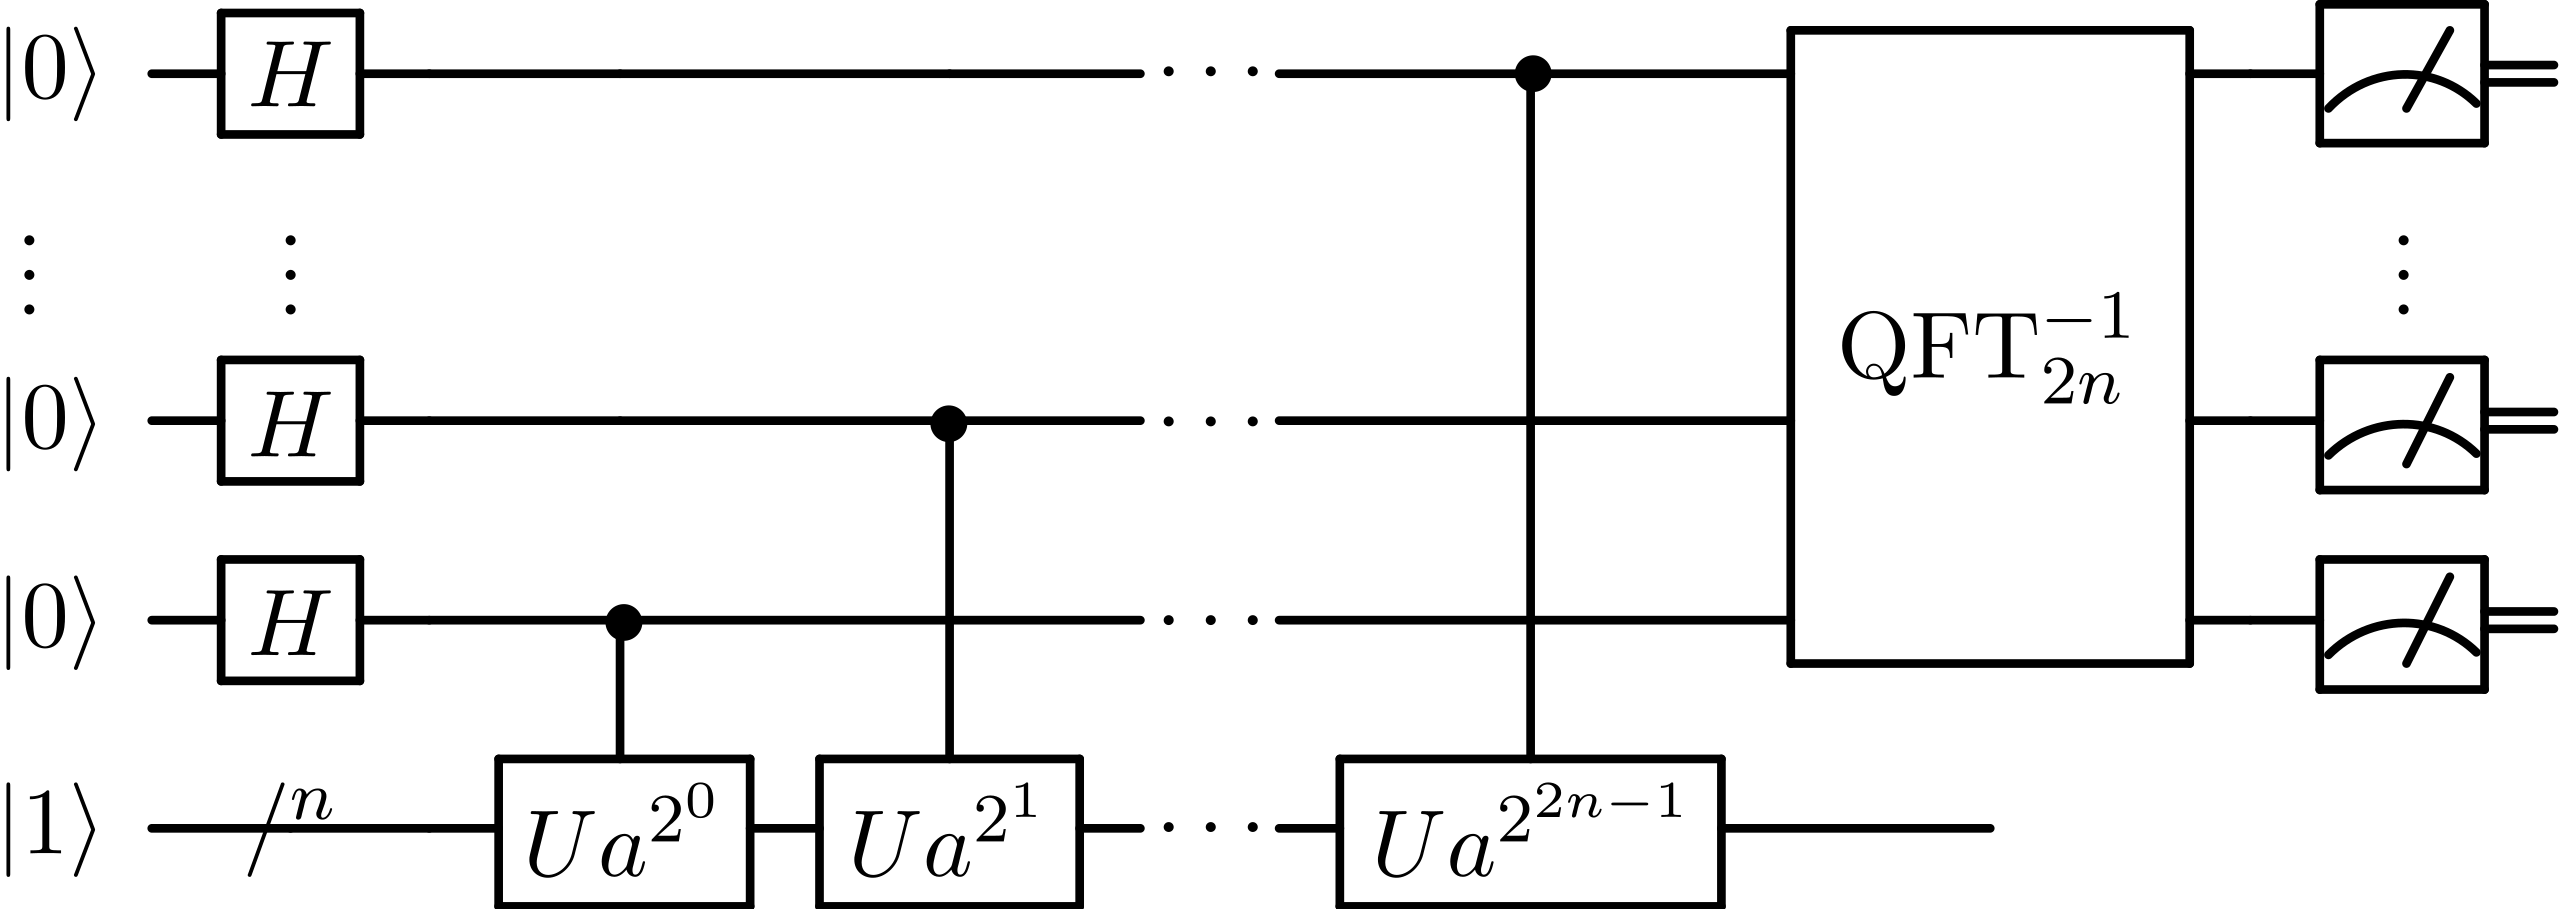
\includegraphics[scale=.15]{images/Shor-QuantumPeriodFinding.png}
    \caption{Period finding quantum subroutine \cite{ShorQuantumSubroutineImage}}
    \label{fig:PeriodFindingQuantumSubroutine}
\end{figure}

Stephane Beauregard\cite{CircuitForShorAlgorithm_2003} provides a detailed description on how the $Ua^{2^k}$ quantum circuits are built.
